\chapter{Directly Interacting with Memory Content}\label{chp:casting}
\epigraph{When I see a bird that walks like a duck and swims like a duck and quacks like a duck, I call that bird a duck.}{James Whitcomb Riley}

In the previous chapter we've seen how we can use C to perform simple computations. The inputs for these computations were given \emph{at compiletime}. That means, once the program was compiled, it would always churn out the same result; we could not reuse the compiled executable to get new results, but always had to edit the code and recompile. In this chapter, we'll use our knowledge about pointers and memory structure to write \emph{interactive} code: programs that take some input from the user \emph{at runtime}, \ie values that were not determined when the code was written. While we're at that, we will also discuss some \enquote{bit magic}, \ie operations that directly take the bitpatterns of the information in memory into account.

\section{Reading Values with \texttt{scanf}}
The command \texttt{scanf} instructs the computer to let the user type some text on the keyboard, interpret it one or another way (\eg as integer or floating point number) and then store it in memory. Unfortunately, we can't instruct the CPU \emph{directly} to store information in a variable. This is because, for the CPU there are no variables -- only memory addresses. Variables are names we give to memory addresses to make life for us humans easier. The compiler knows which variable name belongs to which memory address, but after it has done its job, there are no names left in the compiled machine code -- only numbers. The command \texttt{scanf} invokes such machine code and is therefore incompatible with human language variable names. To do its job (writing a number to memory), we need to provide the \emph{address} of the variable that should store the number.

We are by now very familiar with the fact that the same information can be interpreted in different ways. In the previous chapter, when we learned about \texttt{printf}, we were concerned with the converision rules from binary (information in memroy) to text (information on screen). In a way, \texttt{scanf} is the counterpart to \texttt{printf}: it takes text information from the user and converts it into a bitpattern. With this preface, you will not be surprised to hear that the format strings we already know about make a comeback\footnote{Also maybe you remember that the \texttt{f} in \texttt{printf} stands for \emph{formatted}. It means the same in \texttt{scanf}.}.

\subsection{Simple Usage}
The simplest way to use the command is the following:

\begin{codebox}[Syntax: \texttt{scanf}]
scanf(formatString, pointerToVariable)
\end{codebox}
in which, again:
\begin{itemize}
\setlength\itemsep{0pt}
\item \texttt{formatString} is text comprising of format codes like \texttt{\%d} which tells how to interpret the user input.
\item \texttt{pointerToVariable} is the address of a variable which should be overwritten with the interpreted user input.
\end{itemize}

Let's look at an example and go through it line by line:
\begin{codebox}[interactiveSum.c]
\begin{minted}[linenos]{c}
#include <stdio.h>

int main () {
    int a = 0, b = 0;
    
    printf("Please enter a first number: ");
    scanf("%d", &a);
    printf("Please enter a second number: ");
    scanf("%d", &b);
    
    printf("The sum of the two is %d\n", a + b);
}
\end{minted}
\captionof{code}{Using \texttt{scanf} to read values from the keyboard}
\end{codebox}
\begin{itemize}
\setlength\itemsep{0pt}
\item Line 1 is of course the well known \texttt{include} directive. We knew before that this command allows us to use the \texttt{printf} command; 
	we also get the \texttt{scanf} command from this directive.
\item In line 4 we declare two integer variables and set them to zero.
\item Line 6 prompts the user to enter a number. Note how the format string \emph{does not} end in \texttt{\textbackslash n} here; 
	the cursor remains in the same line as the text just written.
\item The \texttt{scanf} command begins by waiting for user input. Whatever the user may type will appear on screen (directly after \texttt{... first number:}).
	When the user is done entering values (\ie when they hit the \emph{return} key), it will attempt to interpret the input according to the format string.
	The format string is \texttt{"\%d"}, which signifies an integer. If the user input could be interpreted as an integer (the user may also enter \texttt{banana}, 
	which cannot be converted into a number\citationneeded[https://xkcd.com/2070/]), this interpretation is written \emph{to the address} \texttt{\&a}.
\item Lines 8 and 9 repeat the above wiht \texttt{\&b}
\item After this, we can use the previously read values which are now stored in the variables \texttt{a} and \texttt{b} to do regular computations like that in line 11.
\end{itemize}

Consequently, running this code could produce output like this:
\begin{cmdbox}[Possible output: interactiveSum.c]
Please enter a first number: 3 \\
Please enter a second number: 4 \\
The sum of the two is 7
\end{cmdbox}


\begin{plusbox}[Why does \texttt{printf} need no addresses?]
Both, the instructions behind the commands \texttt{printf} and behind \texttt{scanf} are available as compiled code, \ie in machine language. As we've learned before, in this stage, the concept of named variables no longer exists -- there are only memory cells. This is why for \texttt{scanf} we had to provide addresses. But why then can \texttt{printf} work just fine with the variables?
\end{plusbox}
%
\begin{plusbox}[]
We learned that normally, code is executed from top to bottom. Invoking a command (we also say: \emph{calling a function}) actually marks a discontinuity in this order. We jump to an entirely different location in memory to read instructions from there. It is comparable to reading a set of instructions like this:
\begin{itemize}
\setlength\itemsep{0pt}
\item Fetch a sufficiently large cup
\item Fill that cup with tea (see page 666 for how to make tea)
\item Drink the tea
\item Describe the taste of the tea (see page 789 for how to describe taste)
\end{itemize}
After fetching the cup (akin to declaring a variable), we stop reading the current page but jump ahead to page 666. Only when we've finished executing the instructions there, we go back and follow the next instruction -- drink the tea.

The instructions on page 666 will refer to \emph{the prepared cup}. It is of course necessary to know, which of the potentially many cups in your house you fill\footnote{unless you want to risk grabbing a too small espresso cup or accidentally grabbing the one cup your fellow lodger stores their priced toe nail clippings in}, so you need to remember \emph{where you placed the cup you're going to use}. This is alike to the situation with \texttt{scanf} -- it needs to know where to put the result of its work to. In other words, it needs the \enquote{address of the cup}.

The other task -- describing the taste of tea -- does not need to make any changes to the cup. However, it does need the memory of which tea we just drank as input. So, it is sufficient here, to pass this \enquote{value of the cup}, regardless of where it stands.

This idea will be covered in more detail in chapter \ref{chp:funcs}
\end{plusbox}

So we can tell the computer what kind of textual input to expect and how to interpret it. But what if the user does not comply? What, if we tell the computer to expect a \inC{double} value (like \texttt{3.14}), but the user types something that is not a number (like \texttt{banana})? Well, best we try it out:

\begin{codebox}[inputNumber.c]
\begin{minted}[linenos]{c}
#include <stdio.h>

int main () {
    double number = 0.0;

    printf("Please enter a number: ");
    scanf("%lf", &number);

    printf("You entered the number %lf\n", number);
}
\end{minted}
\captionof{code}{Interpreting nonsensical user input (1)}
\end{codebox}

First we check whether the code works as intended by actually entering a number:
\begin{cmdbox}[Possible output: inputNumber.c]
Please enter a number: 3.14 \\
You entered the number 3.140000
\end{cmdbox}

Great. Everything as we expected it. Now let's try to enter something that is not a number:
\begin{cmdbox}[Possible output: inputNumber.c]
Please enter a number: banana \\
You entered the number 0.000000
\end{cmdbox}

We got the result \texttt{0.000000}, which could have two possible reasons:
\begin{itemize}
\item If a user input cannot be interpreted as a number, the computer might default to zero
\item or it might not update the value of the variable (cf line 4: we initialized \texttt{number} to be zero from the start)
\end{itemize}
But which one is it? Let's do another experiment:
\begin{codebox}[inputNumberAlt.c]
\begin{minted}[linenos]{c}
#include <stdio.h>

int main () {
    double number = -1.0;

    printf("Please enter a number: ");
    scanf("%lf", &number);

    printf("You entered the number %lf\n", number);
}
\end{minted}
\captionof{code}{Interpreting nonsensical user input (2)}
\end{codebox}

\begin{cmdbox}[Possible output: inputNumberAlt.c]
Please enter a number: banana \\
You entered the number -1.000000
\end{cmdbox}

With this we come to an conclusive answer to our question: nonsensical input is simply ignored.

\begin{hintbox}[A training in emerging complexity]
So by writing a short piece of code and altering it slightly, we've come to a result we can work with. Of course, it's not really necessary to make experiments to find that out; we could also look up that kind of information in any reference manual. But these examples double as an exercise in the way of thinking that we will adapt over the course of this book: we identified all the factors that could possibly change the value of the variable \texttt{number} and dealt with them.
\end{hintbox}

Implicitly, there's now a new question: can we tell for sure, whether the user has entered a reasonable value for our question? After all, \texttt{0.0} or \texttt{-1.0} are numbers, too. So we can't say: \emph{if the value still has its initial value after the \texttt{scanf} command, the user must have entered something nonsensical}. It turns out that there is a way:

We say that \texttt{scanf} is a function. This name comes from the fact that it behaves like a mathematical function (think, for example, of the sine of an angle) in that it \emph{computes a value}. Changing the content of a variable is only a \emph{side effect}, like with the assignment operator (\texttt{=}) when we discussed the order of operations (cf. section \ref{sec:OrderOfOperations}). That means, in C this code \enquote{makes sense}, \ie can be compiled:
\begin{codebox}[returnValue.c]
\begin{minted}[linenos]{c}
#include <stdio.h>

int main () {
    double number = -1.0;
    int returnValue = -1;
    printf("Please enter a number: ");
    returnValue = scanf("%lf", &number);
    
    printf("You entered: %lf\nThe return value was: %d\n", number, returnValue);
}
\end{minted}
\captionof{code}{Catching the return value of \texttt{scanf}}
\end{codebox}

In line 8, we \enquote{catch} the \emph{return value} of the function. That means, we store the result of the computation in a variable \texttt{returnValue}. In the case of \texttt{scanf}, this return value is an integer and stores the \emph{number of successfully interpreted values}\footnote{In section \ref{sec:ScanfMultiValues}, we will see that we can read more than one value with a single call to \texttt{scanf}.} That means, in the above case it will be \inC{1} if the user input was indeed a number, and \inC{0} otherwise:

\begin{tcbraster}[raster columns=2,
                  raster equal height,
                  nobeforeafter,
                  raster column skip=0.2cm]
\begin{cmdbox}[Possible Output: returnValue.c]
Please enter a number: 2.718 \\
You entered: 2.718000 \\
The return value was: 1
\end{cmdbox}
%
\begin{cmdbox}[Possible Output: returnValue.c]
Please enter a number: banana \\
You entered: -1.000000 \\
The return value was: 0
\end{cmdbox}
\end{tcbraster}

This feature can be used to make a more robust user interface (if the user makes a wrong input, we can tell them to fix their mistake) and can be very handy when debugging (new programmers often pick the wrong format character, which makes the computer incapable of correctly interpreting their input. Catching the return value of \texttt{scanf} is an easy check for that kind of mistake).

\begin{hintbox}[Return value of \texttt{printf}]
Actually, \texttt{printf} is a function, too! It computes the number of characters printed on screen:

\begin{tcbraster}[raster columns=2,
                  raster equal height,
                  nobeforeafter,
                  raster column skip=0.2cm]
\begin{codebox}[printCount.c]
\begin{minted}[linenos]{c}
#include <stdio.h>

int main () {
    int reVal = -1;
    reVal = printf("foo bar\n");
    printf("reVal = %d\n", reVal);
}
\end{minted}
\captionof{code}{Catching the return value of \texttt{printf}}
\end{codebox}
%
\begin{cmdbox}[Possible Output: returnValue.c]
foo bar \\
reVal = 8
\end{cmdbox}
\end{tcbraster}

Indeed, there are \emph{eight} characters on screen: three for \texttt{foo}, one for the whitespace, three for \texttt{bar} and one for the line break \texttt{\textbackslash n} (Otherwise, \texttt{reVal = 8} would end up in the same line as \texttt{foo bar}).
\end{hintbox}

\subsection{The Keyboard Buffer}
So far we've said: \texttt{scanf} reads text from the keyboard, interprets it and writes the interpretation result to memory. Actually, that was a simplification. It is usually sufficient to think of the command in these terms, but to understand some quirks of the command, we should have a closer look. This will help us when debugging our code, as discussed in section \ref{sec:scanfMistakes}.

The code behind the command \texttt{scanf}

%TODO
% what happens in %d @ "12.3" (gives 12, ".3" remains in buffer)

% the %d%c%d disaster...

\subsection{Reading Multiple Values in Sequence} \label{sec:ScanfMultiValues}

\subsection{Common Mistakes} \label{sec:scanfMistakes}
There are a number of mistakes that even experienced coders make from time to time. It is easy to write C-Code that does compile but has an unintended effect. Here, I want to discuss some of the most common mistakes one can make when using \texttt{scanf}.

\subsubsection{Forgetting the Ampersand}
You remember that \texttt{scanf} needs an \emph{address} to write the interpreted value to. You also remember that you get the address of a variable with the ampersand operator (\texttt{\&}).  What would happen, if you forgot that operator?

In a word, the result is \emph{unpredictable}. We also say, \emph{using an invalid address gives undetermined behaviour}. If you forget to use the address operator \texttt{\&}, whatever value was stored in the variable is interpreted as an address. So essentially, you get a random address to which you write. Who can say what this memory location is being used for?

There are three possible scenarios:
\begin{itemize}
\item The random address points to \emph{unused memory}. You write the user input into a random cell that nobody knows about -- the result is \enquote{forgotten}.
	Your target variable is not updated, but the return value from \texttt{scanf} indicates that a value was correctly read.
\item The random address points to \emph{used memory}. You overwrite the value of some variable, but not the one you wanted to change, which remains untouched.
\item The random address points to \emph{forbidden memory}. There are memory sections that can only be changed by certain programs, to ensure a stable system. The operating system
	\emph{watches} each program's activities. If one of them tries to access a forbidden section (\eg the section where the operating system itself resides), it refuses the access and
	shuts the program down. You will see an error message about a \emph{segmentation fault} (often abbreviated to segfault), which is the formal terminus for accessing forbidden memory.\\
	A variation thereof is \emph{stack smashing}. The difference between a segfault and stack smashing is subtle, and understanding it won't help us much.
	Simply remember that both mean \emph{access to forbidden memory}.\\
	Segfaults and Stack Smashing are the most likely outcome of forgetting the ampersand.
\end{itemize}

It actually is difficult to synthesize the first two of the above scenarios; however, we can reliably reproduce \emph{segfaults} and \emph{stack smashing}. Note that the compiler already warns us that we've made a mistake:
\begin{tcbraster}[raster columns=2,
                  raster equal height,
                  nobeforeafter,
                  raster column skip=0.2cm]
\begin{warnbox}[segfault.c, leftupper=7mm]
\begin{minted}[linenos]{c}
#include <stdio.h>

int main () {
    int value = 0;
    
    printf("Enter a value: "); 
    scanf("%d", value);
    
    printf("%d\n", value);
}
\end{minted}
\captionof{code}{Causing a segfault with \texttt{scanf}}
\end{warnbox}
%
\begin{cmdbox}[Output: segfault.c]
\begin{minted}{text}
$ gcc -Wall -Wextra -Wpedantic 
    segfault.c -o segfault
segfault.c: In function ‘main’:
segfault.c:7:13: warning: format ‘%d’ 
    expects argument of type ‘int *’,
    but  argument 2 has type ‘int’ 
    [-Wformat=]
    7 |     scanf("%d", value);
      |            ~^   ~~~~~
      |             |   |
      |             |   int
      |             int *
$ ./segfault
0
Segmentation fault (core dumped)
\end{minted}
\end{cmdbox}
\end{tcbraster}

\vfill
Stack smashing can only occur when the number is an \emph{almonst valid} address, \ie very close to a point in memory that we are allowed to access. Modern computers use 64bit addresses, while an \inC{int} is only a 32bit variable. Hence, the example below uses the data type \inC{long long int}, together with the format string \texttt{\%lld}, which stands for this data type. In its core, the example below has the same structure as the one above. Only the initial value is such an \emph{almost valid} address.

\begin{warnbox}[stackSmashing.c, leftupper=7mm]
\begin{minted}[linenos]{c}
#include <stdio.h>

int main () {
    long long int value = &value + 1;
    
    printf("Enter a value: ");
    scanf("%lld", value);
    
    printf("%lld\n", value);
}
\end{minted}
\captionof{code}{Causing stack smashing with \texttt{scanf}}
\end{warnbox}

Again, the compiler tries to warn us:
\begin{cmdbox}[Output: stackSmashing.c]
\begin{minted}{text}
$ gcc -Wall -Wextra -Wpedantic stackSmashing.c -o stackSmashing
stackSmashing.c: In function ‘main’:
\end{minted}
\end{cmdbox}
%
\begin{cmdbox}[]
\begin{minted}{text}
stackSmashing.c:4:27: warning: initialization of ‘long long int’ from 
    ‘long long int *’ makes integer  from pointer without a cast 
    [-Wint-conversion]
    4 |     long long int value = &value + 1;
      |                           ^
stackSmashing.c:7:15: warning: format ‘%lld’ expects argument of type 
    ‘long long int *’, but argument 2 has type ‘long long int’ [-Wformat=]
    7 |     scanf("%lld", value);
      |            ~~~^   ~~~~~
      |               |   |
      |               |   long long int
      |               long long int *
$ ./stackSmashing
Enter a value: 0
140732161677208
*** stack smashing detected ***: terminated
Aborted (core dumped)
\end{minted}
\end{cmdbox}

\subsubsection{Using the wrong Format String Elements}
As far as the computer is concerned, the \texttt{scanf} command means the following: take some text from the keyboard, convert it into a bitpattern according to rules set out in a format string, and write them to some specified address. This set of instructions does not involve checking whether the bitpattern makes any sense at the target address\footnote{because such a check would not be possible}. If you tell the computer to write a floating point value to an integer address, it will comply -- only that the result is nonsensical (at best). Let's regard two examples:
\begin{tcbraster}[raster columns=2,
                  raster equal height,
                  nobeforeafter,
                  raster column skip=0.2cm]
\begin{warnbox}[typeMismatch.c, leftupper=7mm]
\begin{minted}[linenos]{c}
#include <stdio.h>

int main () {
    double value = 0.0;
    
    printf("Enter a value: "); 
    scanf("%d", &value);
    
    printf("%lf\n", value);
}
\end{minted}
\captionof{code}{Type mismatch with \texttt{scanf}}
\end{warnbox}
%
\begin{cmdbox}[Output: typeMismatch.c]
\begin{minted}{text}
$ gcc -Wall -Wextra -Wpedantic 
    typeMismatch.c -o typeMismatch
$ ./typeMismatch
typeMismatch.c: In function ‘main’:
typeMismatch.c:7:13: warning: format 
    ‘%d’ expects argument of type 
    ‘int *’, but argument 2 has type 
    ‘double *’ [-Wformat=]
    7 |     scanf("%d", &value);
      |            ~^   ~~~~~~
      |             |   |
      |             |   double *
      |             int *
      |            %le
Enter a value: 2.718 
0.000000
\end{minted}
\end{cmdbox}
\end{tcbraster}
Here we told the computer to read an integer (\texttt{\%d}) to a \inC{double} slot. As predicted, the result (\texttt{0.0}) has nothing to do with what we entered (\texttt{2.718}). At least, our trusted friend the compiler warns us again of this mistake.

A somewhat worse version is this:
\begin{tcbraster}[raster columns=2,
                  raster equal height,
                  nobeforeafter,
                  raster column skip=0.2cm]
\begin{warnbox}[bleeding.c, leftupper=7mm]
\begin{minted}[linenos]{c}
#include <stdio.h>

int main () {
    int val1 = -1, val2 = -1;

    printf("Enter a value: ");
    scanf("%lf", &val1);

    printf("value 1 = %d\n", val1);
    printf("value 2 = %d\n", val2);
}
\end{minted}
\captionof{code}{bleeding with \texttt{scanf}}
\end{warnbox}
%
\begin{cmdbox}[Output: bleeding.c]
\begin{minted}{text}
$ gcc -Wall -Wextra -Wpedantic 
    bleeding.c -o bleeding
$ ./bleeding
bleeding.c: In function ‘main’:
bleeding.c:7:14: warning: format 
    ‘%lf’ expects argument of type 
    ‘double *’, but argument 2 has 
    type ‘int *’ [-Wformat=]
    7 |     scanf("%lf", &val1);
      |            ~~^   ~~~~~
      |              |   |
      |              |   int *
      |              double *
      |            %d
Enter a value: 1
value 1 = 0
value 2 = 1072693248
\end{minted}
\end{cmdbox}
\end{tcbraster}

Not only did we not get what we expected for \texttt{val1}; the \texttt{scanf} command also destroyed the information stored in \texttt{val2}!

To understand this, you have to know that \texttt{val1} and \texttt{val2} are (in this example) arranged in memory such they are right next to each other. Each of them is a variable of type \inC{int}, which means it takes up 32 bit or 4 Byte worth of memory. The \enquote{write-command} in \texttt{scanf} tells the computer to write a value of type \inC{double}, which is 64 bits or \emph{eight} bytes: we write over the confines of one \enquote{memory compartment} (the variable \texttt{val1}) and \enquote{bleed} into the next compartment (the variable \texttt{val1}).

\begin{defbox}[Memory Picture]
\begin{center}
\begin{tikzpicture}
  [
    minicell/.style={text width= 3mm, text height=2mm, draw=black, inner sep=1mm},
    widecell/.style={text width=18mm, text height=4mm, draw=black, inner sep=1mm},
    ld/.style={draw=blue,shorten >=2pt,->}
  ]
  
  \node (c0) at (0.0,8) [minicell] {};
  \node (c1) at (0.5,8) [minicell] {};
  \node (c2) at (1.0,8) [minicell] {};
  \node (c3) at (1.5,8) [minicell] {};
  \node (p0) [above=0mm of c0] {\tiny \color{blue} 0x27fb};
  \node (p1) [above=2mm of c1] {\tiny 0x27fc};
  \node (p2) [above=0mm of c2] {\tiny 0x27fd};
  \node (p3) [above=2mm of c3] {\tiny 0x27fe};
  \node (C0) at (0.75,7.5) [widecell] {\texttt{val1}};
  
  \node (c4) at (2.0,8) [minicell] {};
  \node (c5) at (2.5,8) [minicell] {};
  \node (c6) at (3.0,8) [minicell] {};
  \node (c7) at (3.5,8) [minicell] {};
  \node (p4) [above=0mm of c4] {\tiny 0x27ff};
  \node (p5) [above=2mm of c5] {\tiny 0x2800};
  \node (p6) [above=0mm of c6] {\tiny 0x2801};
  \node (p7) [above=2mm of c7] {\tiny 0x2802};
  \node (C1) at (2.75,7.5) [widecell] {\texttt{val2}};
  
  \node (c8) at (4.0,8) [minicell] {};
  \node (c9) at (4.5,8) [minicell] {};
  \node (cA) at (5.0,8) [minicell] {};
  \node (cB) at (5.5,8) [minicell] {};
  \node (p8) [above=0mm of c8] {\tiny 0x2803};
  \node (p9) [above=2mm of c9] {\tiny 0x2804};
  \node (pA) [above=0mm of cA] {\tiny 0x2805};
  \node (pB) [above=2mm of cB] {\tiny 0x2806};
  \node (C2) at (4.75,7.5) [widecell] {...};
  
  \node (cC) at (6.0,8) [minicell] {};
  \node (cD) at (6.5,8) [minicell] {};
  \node (cE) at (7.0,8) [minicell] {};
  \node (cF) at (7.5,8) [minicell] {};
  \node (pC) [above=0mm of cC] {\tiny 0x2807};
  \node (pD) [above=2mm of cD] {\tiny 0x2808};
  \node (pE) [above=0mm of cE] {\tiny 0x2809};
  \node (pF) [above=2mm of cF] {\tiny 0x280A};
  \node (C2) at (6.75,7.5) [widecell] {...};  

  \node (lblCells)     at (-2, 8.0) {memory cells};
  \node (lblCompounds) at (-2, 7.5) {variables};
  \node (lblAddress)   at (-2, 8.5) {address of \texttt{val1}};
  
  \draw [ld] (lblAddress.east) .. controls +(0.3,0) .. (p0.west);
  \draw [
	    thick,
	    decoration={
	        brace,
	        %mirror,
	        raise=1.0cm
	    },
	    decorate
	] (c0.west) -- (c7.east) 
node [pos=0.5,anchor=north,yshift=+1.7cm] {eight bytes for a \texttt{double} value}; 
\end{tikzpicture}
\end{center}
\captionof{figure}{Bleeding}
\end{defbox}

\begin{hintbox}[Double-check your pointer assignments]
As you've seen, not only can you get nonsensical data if you mix up the format strings and the variables that are written with these format strings; you can also destroy other values. As you can imagine, this makes debugging exceedingly difficult (try finding the point in the code that changes \texttt{val2}, if nothing in it seems to even touch it). It is therefore of utmost importance that you are always aware of the data types of the values that you want to write and the means by which you do so. This holds particularly for working with pointers.
\end{hintbox}

\subsubsection{Non-Placeholder Characters in the Format String}
When typing a \texttt{printf} format string, we pretty much always put a line break (\texttt{\textbackslash n}) at its end. It almost becomes an automatism. It is no surprise thus that, in my time as a teacher, I've seen several students putting the same sequence, and I can't blame them for their mistake\footnote{which is infuriatingly hard to spot.}. So, again, let's consider an example and see what happens if we compile and run it:

\begin{tcbraster}[raster columns=2,
                  raster equal height,
                  nobeforeafter,
                  raster column skip=0.2cm]
\begin{warnbox}[linebreakScanf.c, leftupper=7mm]
\begin{minted}[linenos]{c}
#include <stdio.h>

int main () {
    int val1 = -1, val2 = -1;

    printf("Enter a value: ");
    scanf("%d\n", &val1);

    printf("Enter another value: ");
    scanf("%d\n", &val2);

    printf("value 1 = %d\n", val1);
    printf("value 2 = %d\n", val2);
}
\end{minted}
\captionof{code}{Line break in format string of \texttt{scanf}}
\end{warnbox}
%
\begin{cmdbox}[Output: linebreakScanf.c]
\begin{minted}{text}
Enter a value: 1
2
Enter another value: 3
value 1 = 1
value 2 = 2
\end{minted}
\end{cmdbox}
\end{tcbraster}

At first, everything looks okay -- no compiler warnings. We can execute and run our code, and up to line 6 everything looks normal. Then we hit the \texttt{scanf} statement, which allows us to enter a value (in this case \texttt{1}). Strangely, though, after that we are not prompted to enter another value (line 9). Instead, the terminal allows us to directly enter \texttt{2}. Only then, line 9 is executed, \ie we are prompted to enter another value. However, when we get to lines 12 and 13, we see that this input has seemingly been ignored, and instead, the value \texttt{2} got into \texttt{val2}, even before line 10 (the only line writing to the address of \texttt{val2}) was exectued.

%TODO
How is this possible? You'll have to read the next section for some of the details; in essens, however, you can think of the line break as the format string equivalent of \enquote{put one value on hold}. 


% what happens if we put line breaks or other non-format chars in there

% note: less user friendly


\section{Casting}


%TODO
% C4 becomes: casting, promotion, scanf, bit magic

% Exo: ask user for two int: number and bit ID; tell if set or not

% ----------------------------------

%Damit ein Prozessor eine Information verarbeiten kann, muss diese in Form von Ketten aus 1 und 0 vorliegen -- also in \emph{binärer} Form. Aus einer Reihe von Bits geht jedoch nicht hervor, ob diese nun als Zahl, Text, Bild, \ldots interpretiert werden sollen\footnote{Da jede digitalisierbare Information auch als Zahl interpretiert werden kann, kommt es zu der bizarren Situation, dass manche (sehr große) Zahlen urheberrechtlich geschützte Werke beschreiben. Insbesondere ist es möglich, solche Zahlen als Primzahlen zu konstruieren. Diese Zahlen werden in Fachkreisen \emph{Illegale Primzahlen} genannt. Ob die gefundenen Primzahlen tatsächlich als illegal gelten, wurde bislang nicht vor Gericht verhandelt.}. In C (und den damit verwandten Sprachen) muss daher zu jeder Information ein \emph{Datentyp} mit angegeben werden\footnote{Andere Sprachen wie etwa Python versuchen, aus dem Kontext zu \enquote{erraten}, welche Art Information vorliegt. Bezug nehmend auf das Zitat zu Eingang des Kapitels nennt man solche Sprachen \emph{duck typed}. C dagegen ist \emph{strong typed}. Die Meinungen zu \emph{Duck-Typing} gehen teils weit auseinander und werden bisweilen recht emotional diskutiert.}.
%
%Wir wollen uns hier vertieft mit der Datenstruktur von Zahlen im Speicher beschäftigen, um im weiteren die Arbeitsweise vieler Befehle genau zu verstehen.
%
%\section{Daten im Speicher}
%\subsection{Wertemenge und Vorzeichen bei Zahlen}\label{sec:DataRepresentation}
%\label{sec:Datawidth}
%In Abschnitt \ref{sec:BinaryNumbers} haben wir bereits gesehen wie positive Ganzzahlen und Schriftzeichen als binäre Werte dargestellt werden können. Ein Prozessor kann i.d.R. jedoch nur Einheiten von je 8 Bits (also ganze \emph{Bytes}) bzw. $2^n\cdot8$ Bits behandeln. Eine Gruppe aus 8 Bits kann einen von $2^8 = 256$ Werten darstellen, also beispielsweise den Zahlenbereich von 0 bis 255. Soll mit größeren Werte gearbeitet werden, müssen mehrere Bytes zu einer Einheit zusammengefasst werden. Zwei Bytes (16 Bits) erlauben also $2^{16} = 65\,536$ verschiedene Werte, bei 4 Bytes (32 Bits) sind dies bereits $2^{32} = 4\,294\,967\,296$ verschiedene Werte. Natürlich muss dem Compiler mitgeteilt werden, wie viele Bytes zu einer Einheit zusammengefasst werden. Dies geschieht über den \emph{Datentyp}. Wir haben bereits den Datentyp \mintinline{c}{int} kennengelernt. Eine Variable vom Typ \mintinline{c}{int} ist eine Ganzzahl, deren genaue Größe von der \emph{Architektur des Zielsystems} abhängt, also von der Art des Rechners, auf dem der Compiler läuft. Der Compiler entscheidet hier also, um ein möglichst effizient laufendes Programm zu erstellen. Üblicherweise werden \mintinline{c}{int}s als 32-bit-Variablen umgesetzt; für bestimmte Microcontroller oder ältere Prozessoren kann dies aber auch als 16-bit-Wert interpretiert werden. Neben \mintinline{c}{int} gibt es außerdem noch \mintinline{c}{short int} (16 bit), \mintinline{c}{char} (8 bit), \mintinline{c}{long int} (32 bit, auch auf älteren Prozessoren), und \mintinline{c}{long long int} (64 bit). Wo es wichtig ist, die \emph{Registerbreite} einer Ganzzahl-Variable exakt zu kennen, stehen noch andere Datentypen zur Verfügung -- Siehe die Tabellen \ref{tab:DatatypesStd} und \ref{tab:DatatypesExt} im Anhang.
%
%Negative Zahlen werden durch die Behandlung des Bits mit der höchsten Wertigkeit als \emph{Vorzeichen-Bits} dargestellt. Das bedeutet, dass ein Bit die Information positiv/negativ enthält anstatt zum normalen Teil der Zahl zu gehören. Um zu vermeiden, dass es eine \enquote{positive Null} gibt, die verschieden von der \enquote{negativen Null} ist, wird die Wertigkeit des Vorzeichenbits von der gesamten Zahl abgezogen. Dieses schwierig in Worte zu fassende Konzept wird klarer, wenn wir es anhand eines Beispiels betrachten:
%
%\begin{tcolorbox}
%	[title=Darstellung einer vorzeichenbehafteten Zahl,
%	 arc=0pt,
%	 outer arc=0pt
%	]
%\begin{center}
%\begin{tikzpicture}[
%  flow/.style={draw=black,->,shorten >=2pt}
%]
%  \node (s7) at (0, 4.3) {\tiny 7};
%  \node (s6) at (1, 4.3) {\tiny 6};
%  \node (s5) at (2, 4.3) {\tiny 5};
%  \node (s4) at (3, 4.3) {\tiny 4};
%  \node (s3) at (4, 4.3) {\tiny 3};
%  \node (s2) at (5, 4.3) {\tiny 2};
%  \node (s1) at (6, 4.3) {\tiny 1};
%  \node (s0) at (7, 4.3) {\tiny 0};
%
%  \node (n7) at (0, 4) {1};
%  \node (n6) at (1, 4) {0};
%  \node (n5) at (2, 4) {1};
%  \node (n4) at (3, 4) {0};
%  \node (n3) at (4, 4) {1};
%  \node (n2) at (5, 4) {0};
%  \node (n1) at (6, 4) {1};
%  \node (n0) at (7, 4) {0};
%
%  \node (e7) at (8.5, 0.0) {$\mathtt{-1 \times 2^7 = -128}$};
%  \node (e6) at (8.5, 0.5) {$\mathtt{ 0 \times 2^6 = ~~~0}$};
%  \node (e5) at (8.5, 1.0) {$\mathtt{ 1 \times 2^5 = ~~32}$};
%  \node (e4) at (8.5, 1.5) {$\mathtt{ 0 \times 2^4 = ~~~0}$};
%  \node (e3) at (8.5, 2.0) {$\mathtt{ 1 \times 2^3 = ~~~8}$};
%  \node (e2) at (8.5, 2.5) {$\mathtt{ 0 \times 2^2 = ~~~0}$};
%  \node (e1) at (8.5, 3.0) {$\mathtt{ 1 \times 2^1 = ~~~2}$};
%  \node (e0) at (8.5, 3.5) {$\mathtt{ 0 \times 2^0 = ~~~0}$};
%
%  \draw[flow] (n7.south) |- (e7.west);
%  \draw[flow] (n6.south) |- (e6.west);
%  \draw[flow] (n5.south) |- (e5.west);
%  \draw[flow] (n4.south) |- (e4.west);
%  \draw[flow] (n3.south) |- (e3.west);
%  \draw[flow] (n2.south) |- (e2.west);
%  \draw[flow] (n1.south) |- (e1.west);
%  \draw[flow] (n0.south) |- (e0.west);
%\end{tikzpicture}
%\end{center}
%\end{tcolorbox}
%Für die Bits 0 bis 6 ändert sich nichts an der Interpretation, die bereits in Abschnitt \ref{sec:BinaryNumbers} besprochen wurde. Lediglich das Bit 7 wird nun als Vorzeichenbit interpretiert und erhält somit seine \emph{negative Wertigkeit}. Es ergibt sich ein Wert von $-128 + 32 + 8 + 2 = -86$.
%
%\mintinline{c}{int}s sind \emph{vorzeichenbehaftet}. Will man nur positive Zahlen speichern, kann man bei der Deklaration der Variablen den \emph{Modifier} \mintinline{c}{unsigned} benutzen:
%\begin{codebox}[Beispiel: Deklaration einer vorzeichenlosen Ganzzahl]
%\begin{minted}[linenos]{c}
%int main () {
%   unsigned int positiv = 9;
%}
%\end{minted}
%\end{codebox}
%
%Was geschieht nun, wenn man einer \mintinline{c}{unsigned}-Variable einen negativen Wert zuweisen will? Betrachten wir das Beispiel:
%\begin{codebox}[Beispiel: Zuweisung einer negativen Zahl zu einer unsigned-Variable]
%\begin{minted}[linenos]{c}
%int main () {
%   unsigned char positiv = -1;
%}
%\end{minted}
%\end{codebox}
%Hier wird der Compiler zuerst das Bitmuster der Zahl \texttt{-1} mit einer Breite von 8 Bit erzeugen, da ein \mintinline{c}{char} geschrieben werden soll. Dieses Bitmuster lautet \texttt{11111111}. Da die Variable \texttt{positiv} aber ein \mintinline{c}{unsigned char} ist, wird dieses Bitmuster nun als positive Zahl interpretiert und im Folgenden als \texttt{255} gelesen.
%
%Für die Darstellung von Kommazahlen (in der Literatur meist \emph{Fließkommazahlen} genannt) stehen die Datentypen \mintinline{c}{float} (32 bit), \mintinline{c}{double} (64 bit) und \mintinline{c}{long double} (80 bit) zur Verfügung, die im Detail selten verstanden werden müssen. Durch die größere Datenmenge bei \mintinline{c}{double}s und \mintinline{c}{long double}s fallen Rundungsfehler bei der Arbeit mit diesen Typen weniger ins Gewicht, jedoch sind Berechnungen hier zeitaufwändiger. In den meisten Fällen ist \mintinline{c}{double} der am besten geeignetste Datentyp beim Umgang mit Fließkommazahlen.
%
%Es gibt keine vorzeichenlosen Fließkommazahlen.
%
%KursteilnehmerInnen, die sich weiter für den Aufbau von Fließkommawerten interessieren, können nach dem Stichwort \emph{Standard IEEE 754} suchen. Insbesondere finden Sie unter der Adresse \url{https://steve.hollasch.net/cgindex/coding/ieeefloat.html} eine einsteigerfreundliche Erklärung. Im Kurs \emph{Numerik} der Universität Regensburg wird die Darstellung von Fließkommazahlen ebenfalls behandelt.
%
%
%\subsection{Adressierung -- Pointer} \label{sec:Pointer}
%Man kann sich den Arbeitsspeicher als langes Band von kleinen, nummerierten Speicherzellen vorstellen. Jede Zelle fässt genau ein Byte. Um einen Wert zu lesen oder zu schreiben muss dem Prozessor die Nummer der Zelle mitgeteilt werden, die verändert wird. Diese Nummer wird \emph{Adresse} oder \emph{Pointer} genannt. Wenn wir im Code Variablen benutzen, übersetzt der Compiler diese in Adressen. Für die einfachsten Aufgaben kann der Compiler die Speicherverwaltung komplett übernehmen. Wir werden jedoch schon in Kapitel \ref{chp:Input} Situationen kennen lernen, wo wir diese Speicherstruktur kennen müssen.
%
%\begin{tcolorbox}[title=Speicherbild]
%\begin{center}
%\begin{tikzpicture}
%  [
%    cell/.style={text width=8mm,
%      text height=4mm, draw=black, inner sep=1mm},
%    ld/.style={draw=blue,shorten >=2pt,->}
%  ]
%  \node (c1) at (0,0) [cell] {\ttfamily 99};
%  \node (c2) at (1,0) [cell] {\ttfamily 1};
%  \node (c3) at (2,0) [cell] {\ttfamily 255};
%  \node (c4) at (3,0) [cell] {\ttfamily 0};
%  \node (c5) at (4,0) [cell] {\ttfamily 80};
%  \node (c6) at (5,0) [cell] {\ttfamily ...};
%
%  \node (labelMem) at (8,  1) {Symbole im Code};
%  \node (labelMem) at (8,  0) {Werte im Speicher};
%  \node (labelMem) at (8, -1) {Adressen};
%
%  \node (a1) [below=2mm of c1]            {\tiny 0x27ff};
%  \node (a2) [below=2mm of c2, color=red] {\tiny 0x2800};
%  \node (a3) [below=2mm of c3]            {\tiny 0x2801};
%  \node (a4) [below=2mm of c4]            {\tiny 0x2802};
%  \node (a5) [below=2mm of c5]            {\tiny 0x2803};
%  \node (a6) [below=2mm of c6]            {\tiny 0x2804};
%
%  \node (ptr) [below=8mm of c1] {\scriptsize Adresse von \texttt{x}};
%  \node (vc2) [above=6mm of c1] {\scriptsize Variable \texttt{x}};
%  \node (vc0) [above=2mm of c1] {\scriptsize Variable \texttt{y}};
%
%  \draw [ld] (ptr.east) .. controls +(0.3,0) .. (a2.south);
%  \draw [ld] (vc0.east) .. controls +(0.4,0) .. (c2.north);
%  \draw [ld] (vc2.east) .. controls +(2.4,0) .. (c4.north);
%\end{tikzpicture}
%\end{center}
%\end{tcolorbox}
%
%Adressen sind Zahlen und können damit auch im Speicher als binäre Werte abgebildet werden. Abhängig von der \emph{Prozessorarchitektur} handelt es sich dabei um 32-bit oder 64-bit Ganzzahlen. Meist werden diese nicht als \emph{Dezimalzahlen}, sondern als \emph{Hexadezimalzahlen} angegeben (\ie mit den \enquote{Ziffern} \texttt{0, 1, 2, 3, 4, 5, 6, 7, 8, 9, A, B, C, D, E, F}. Siehe Abschnitt \ref{sec:NumSystems} für weitere Details hierzu.
%
%Neben der Information, wo im Speicher eine bestimmte Information liegt, muss natürlich auch bekannt sein, wie diese zu interpretieren ist. Daher wird an dieser Stelle zu jedem Datentyp ein zugehöriger \emph{Pointer} eingeführt, also ein Datentyp, der die Adresse einer Information enthält.
%
%Pointer können ebenfalls in Variablen gespeichert werden. Die Deklaration erfolgt wie schon in Abschnitt \ref{sec:DeclareVars}. Der einzige Unterschied ist, dass ein Pointer-Typ gegenüber seinem \emph{Basistyp} durch ein Sternchen \texttt{*} ausgezeichnet wird.
%
%\begin{codebox}[Beispiel: Deklaration von Pointer-Variablen]
%\begin{minted}[linenos]{c}
%int main () {
%   int   normaleVariable;
%   int * pointer;
%}
%\end{minted}
%\end{codebox}
%
%Um die Adresse anderer Variablen in Erfahrung zu bringen bedienen wir uns des Adress-Operators \texttt{\&}:
%
%\begin{codebox}[Beispiel: Deklaration von Pointer-Variablen]
%\begin{minted}[linenos]{c}
%int main () {
%   int   normaleVariable;
%   int * pointer = &normaleVariable;
%}
%\end{minted}
%\end{codebox}
%
%Wir sagen also, \texttt{pointer} \enquote{zeigt auf} \texttt{normaleVariable}, \ie in der Variablen \texttt{pointer} ist die Information gespeichert, wo \texttt{normaleVariable} im Speicher zu finden ist.
%
%Pointer können \emph{dereferenziert} werden; das heißt, anstatt mit der Adresse selbst zu arbeiten, behandeln wir den Wert, auf den der Pointer zeigt. Dies kann sowohl lesend als auch schreibend stattfinden. Wir benutzen den \emph{Dereferenzierungs-Operator} \texttt{*}:
%
%\begin{codebox}[Beispiel: Dereferenzierung eines Pointers]
%\begin{minted}[linenos]{c}
%#include <stdio.h>
%
%int main () {
%   int   normaleVariable = 5;
%   int * pointer = &normaleVariable;
%
%   printf("normaleVariable = %d\n", normaleVariable);
%   printf("*pointer        = %d\n", *pointer);
%   printf("Adresse von normaleVariable: %p\n", pointer);
%
%   *pointer = 8;
%   printf("normaleVariable = %d\n", normaleVariable);
%}
%\end{minted}
%\end{codebox}
%
%Wir legen zuerst eine normale Variable mit Wert \texttt{5} an, sowie einen Pointer, der auf diese Variable zeigt. Wenn über den \emph{dereferenzierten Pointer} \texttt{*pointer} in Zeile 8 ein lesender Zugriff stattfindet, passiert genau dasselbe, als würde direkt mit der Variablen \texttt{normaleVariable} selbst gearbeitet werden: \texttt{printf} liest den Wert \texttt{5} aus dem Speicher.
%Ebenso ändert auch der Zugriff über \texttt{*pointer} in Zeile 11 tatsächlich den Wert von \texttt{normaleVariable}. Die Ausgabe des Wertes von \texttt{pointer} selbst (also ohne Dereferenzierungs-Operator \texttt{*}) in Zeile 9 liefert eine große Zahl in Hexadezimal-Darstellung, die mit dem \emph{Wert} von \texttt{normaleVariable} nichts zu tun hat.
%
%Folglich lautet die Ausgabe:
%
%\begin{cmdbox}[Ausführungsbeispiel: Dereferenzierung eines Pointers]
%\begin{minted}{text}
%normaleVariable = 5
%*pointer        = 5
%Adresse von normaleVariable: 0x7ffdea635c5c
%normaleVariable = 8
%\end{minted}
%\end{cmdbox}
%
%\begin{warnbox}[Große Bedeutung von Pointern in C]
%In der Sprache C ist der Umgang mit Pointern üblich, aber zugleich auch eine der größten Fehlerquellen. Verinnerlichen Sie daher die soebenen gezeigten Konzepte; wir werden hierauf immer wieder aufbauen.
%\end{warnbox}
%
%\FloatBarrier
%\begin{figure}
%\begin{center}
%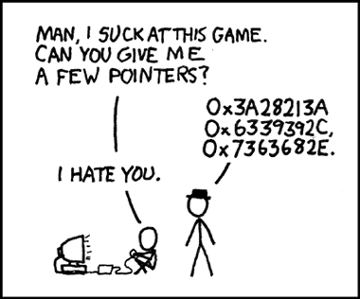
\includegraphics[width=.5\linewidth]{./gfx/xkcd-pointers}
%\caption[Pointer im echten Leben]{Pointer im echten Leben. Quelle: \url{https://xkcd.com/138/}}
%\end{center}
%\end{figure}
%\FloatBarrier
%
%\begin{plusbox}
%Während C++ ebenfalls Pointer zur Verfügung stellt, die sich dort genauso verhalten wie in der Sprache C, gilt das Paradigma, in C++ \emph{keine} Pointer zu verwenden. C++ kennt andere Konzepte, die Pointer ersetzen (bzw. verstecken) und die helfen, häufige Fehler bei der Arbeit mit Pointern zu vermeiden. Im Rahmen dieses Kurses können leider nur Stichworte genannt werden; sehen Sie dies als Motivation, einen C++-Kurs zu besuchen.
%
%Auch wenn C++-Code \idR keine Verwendung von Pointern macht ist die Kenntnis des Konzepts auch dort sehr wichtig, da der gesamte \enquote{Unterbau} der Sprache auf den hier präsentierten Techniken beruht.
%\end{plusbox}
%
%\section{Bitweise Logik und Bit-Shifting} \label{sec:BitwiseOperator}
%Für Elektronik-Anwendungen ist es oft nötig, einzelne Schalter an- oder auszuschalten. Meist geschieht dies über eine Zustandsvariable, die an einen \emph{Port} (ein Anschluss, über den Daten fließen können) gesendet wird. Diese Zustandsvariable ist dann \idR eine Ganzzahl-Variable, in der jedes Bit für einen eigenen Schalter steht. Wir benötigen also Mittel, um einzelne Bits zu manipulieren.
%
%Dazu stehen uns die Operatoren \texttt{\~}, \texttt{\&}, \texttt{|}, \texttt{\^}, \texttt{<{}<} und \texttt{>{}>} zur Verfügung.
%
%Die \emph{bitweise Negation} (NOT, auch \emph{1er Komplement} genannt) \texttt{\~} kehrt jedes Bit um. Betrachten wir die vorzeichenlose 8-Bit-Zahl \texttt{42} (\texttt{00101010}). Das Ergebnis der Negation ist der Wert \texttt{213} (Binärzahl \texttt{11010101}). Als Code lässt sich das wie folgt umsetzen:
%\begin{codebox}[Beispiel: Bitweise Negation]
%\begin{minted}[linenos]{c}
%int main () {
%   unsigned char source = 42;
%   unsigned char result = ~source;
%}
%\end{minted}
%\end{codebox}
%
%Das \emph{bitweise und} (AND) \texttt{\&} vergleicht die Bits von zwei Werten und setzt das Bit im Ergebnis nur, wenn beide Bits in den Vergleichswerten gesetzt waren (\ie den Wert 1 hatten).
%
%Beim \emph{bitweisen oder} (OR) \texttt{|} werden ebenfalls die Bits von zwei Werten verglichen. Das entsprechende Bit im Ergebnis wird jedoch bereits gesetzt, wenn mindestens eines der Vergleichsbits gesetzt war.
%
%Das \emph{bitweise ausschließliche oder} (XOR) \texttt{\^} arbeitet genauso wie das OR, setzt das Ergebnis-Bit jedoch nur, wenn \emph{genau} eines der Vergleichsbits gesetzt war.
%
%All dies lässt sich in den folgenden Wahrheits-Tabellen ausdrücken:
%\begin{codebox}[Wahrheitstabellen: Bitweise Operatoren]
%\begin{minted}{text}
%     1 1 0 0   12       1 1 0 0   12       1 1 0 0   12
%     1 0 1 0   10       1 0 1 0   10       1 0 1 0   10
%     - AND -   --       -- OR -   --       - XOR -   --
%     1 0 0 0    8       1 1 1 0   14       0 1 1 0    6
%\end{minted}
%\end{codebox}
%
%Als Code lässt sich das wie folgt umsetzen:
%\begin{codebox}[Beispiel: Bitweise Operatoren]
%\begin{minted}[linenos]{c}
%int main () {
%   unsigned char lhs = 12, rhs = 10,
%                 and, or, xor;
%   and = lhs & rhs;    // =  8
%   or  = lhs | rhs;    // = 14
%   xor = lhs ^ rhs;    // =  6
%}
%\end{minted}
%\end{codebox}
%
%Die Negation benötigt nur ein \emph{Argument} (Wert, mit dem gearbeitet wird), und wird daher \emph{unärer Operator} genannt. Für AND, OR und XOR sind zwei Werte nötig, weswegen diese als \emph{binäre Operatoren} bezeichnet werden. Die Argumente können auch komplexe Ausdrücke sein, also Ergebnisse von Berechnungen:
%\begin{codebox}[Beispiel: Bitweise Operatoren]
%\begin{minted}[linenos]{c}
%int main () {
%   unsigned char result = ~(2 + 7 * (18 & 5));
%}
%\end{minted}
%\end{codebox}
%
%Bitmuster können als ganzes nach links oder rechts verschoben werden. Hierzu dienen die Operatoren \texttt{<{}<} und \texttt{>{}>}.
%\begin{codebox}[Beispiel: Bitweise Operatoren]
%\begin{minted}[linenos]{c}
%int main () {
%   unsigned char toLeft  = 170 << 1;
%   unsigned char toRight =  85 >> 1;
%}
%\end{minted}
%\end{codebox}
%Dies löst folgende Veränderung aus:
%\begin{codebox}[Bitshift nach links bzw. nach rechts um jeweils eine Stelle]
%\begin{minted}{text}
%     1 0 1 0 1 0 1 0   170       0 1 0 1 0 1 0 1    85
%     ----- << 1 ----   ---       ----- >> 1 ----   ---
%     0 1 0 1 0 1 0 0    84       0 0 1 0 1 0 1 0    42
%\end{minted}
%\end{codebox}
%Bei einem Bitshift nach links werden die Bits am rechten Ende des Bitmusters mit nullen aufgefüllt.
%%Stellen, die am linken Ende über die Registerbreite der aufnehmenden Variable hinaus verschoben werden, gehen verloren.
%Stellen, die über das linke Ende hinaus verschoben werden, gehen verloren.
%Alles eben gesagte gilt analog für den Bitshift nach rechts.
%
%\begin{hintbox}[Multiplikation mit Zweierpotenzen]
%Ein Bitshift um \texttt{n} Stellen nach links entspricht der Multiplikation mit der Zahl $2^{n}$.
%Ein Bitshift um \texttt{n} Stellen nach rechts entspricht der Division durch die Zahl $2^{n}$ (Bei Ergebnissen mit Nachkommastelle wird abgerundet). Bitshifts werden schneller durchgeführt als Multiplikationen mit \texttt{*}.
%
%Dies gilt nur für Ganzzahlen, nicht aber für Fließkommazahlen.
%\end{hintbox}
%
%\section{Typecasting} \label{sec:Casting}
%Es ist gelegentlich notwendig, einen Wert von einem Datentyp in einen anderen umzuwandeln. Bei einer solchen Umwandlung kann sich das Bitmuster ändern, beispielsweise wenn die Ganzzahl \texttt{3} in die Fließkommazahl \texttt{3.0} umgewandelt wird.
%
%Eine solche Umwandlung wird als \emph{Typecasting} bezeichnet. Die Syntax hierzu ist simpel:
%\begin{codebox}[Syntax: Typecasting]
%\texttt{(Ziel-Datentyp) Ausdruck}
%\end{codebox}
%\texttt{Ziel-Datentyp} ist ein beliebiger Datentyp, wie beispielsweise in Anhang \ref{sec:Datatypes} beschrieben. Wie üblich kann \emph{Ausdruck} ein einfacher Wert, eine Variable oder ein komplexer Ausdruck sein.
%
%Ein Grund, den Datentyp zu ändern wurde zum Ende von Abschnitt \ref{sec:OperatorsArithmetic} bereits angeprochen: Operationen wie die Division verhalten sich unterschiedlich, abhängig davon, ob eine Fließkommazahl oder eine Ganzzahl an der Operation beteiligt ist. Solche \emph{Datentyp-spezifischen} Szenarios sind in C sehr häufig.
%
%\begin{codebox}[Beispiel: Typecasting int zu double]
%\begin{minted}[linenos]{c}
%int main () {
%   int x = 7, y = 5;
%   double z = (double) x / y;
%}
%\end{minted}
%\end{codebox}
%
%\begin{hintbox}[Reihenfolge der Operationen]
%Der Compiler arbeitet \enquote{von links nach rechts}, beachtet aber, dass manche Operationen \enquote{Vorrang} vor anderen haben (\eg Punkt-vor-Strich). Im obigen Beispiel wird also zuerst der Typecast der Variablen \texttt{x} durchgeführt, und dann der zum \mintinline{c}{double} konvertierte Wert von \texttt{x} durch \texttt{y} geteilt. Damit erhält \texttt{z} den Wert \texttt{1.2}.
%
%Im folgenden Beispiel dagegen erhält \texttt{z} den Wert 1.0:
%\begin{codebox}[Beispiel: Fehlerhaftes Typecasting int zu double]
%\begin{minted}[linenos]{c}
%int main () {
%   int x = 7, y = 5;
%   double z = (double) (x / y);
%}
%\end{minted}
%\end{codebox}
%Durch die Klammern interpretiert der Compiler Zeile 3 als: \enquote{Caste das Ergebnis von \texttt{x / y} zu \mintinline{c}{double}}. Da das Ergebnis von \texttt{x / y} aus der Division zweier \mintinline{c}{int}-Werte hervorgeht, wird hier gerundet und \texttt{z} erhält den (\idR falschen) Wert \texttt{1.0}.
%\end{hintbox}
%
%\section{Hierarchie der Operatoren} \label{sec:OperatorHierarchy}
%Ausdrücke werden vom Compiler \enquote{von links nach rechts} ausgewertet, wobei die Vorrangigkeit mancher Operatoren beachtet wird. Die Vorrangigkeit kann Tabelle \ref{tab:OperatorPrecedence} im Anhang entnommen werden. Wo immer Unsicherheiten bestehen, kann durch Setzen von (runden Klammern) Sicherheit geschaffen werden.
%
%\section{Zahlenformate -- Hexadezimalsystem} \label{sec:NumSystems}
%Gleich zu Beginn dieses Kurses in Abschnitt \ref{sec:BinaryNumbers} haben wir das \emph{Binärsystem} (oder auch \emph{Dualsystem}) kennen gelernt, das neben dem uns vertrauten \emph{Dezimalsystem} steht\footnote{Übrigens: Das Dezimalsystem wäre völlig unbrauchbar, wenn der Mensch nicht zufällig zehn Finger hätte. (Kalenderspruch)}. Nach der dort gezeigten Idee lassen sich Zahlen in beliebigen \emph{Zahlensystemen} bzw. mit beliebiger \emph{Basis} (also Anzahl von verschiedenen Ziffern im Zahlensystem) darstellen. Von besonderer Bedeutung ist das \emph{Hexadezimalsystem} mit 16 Ziffern:
%
%\begin{center}
%\texttt{0 1 2 3 4 5 6 7 8 9 A B C D E F}
%\end{center}
%
%Um eine Zahl als \emph{hexadezimal} zu kennzeichnen wird häufig der Präfix \texttt{0x} vorangestellt. Der Ausdruck\footnote{Andere verbreitete Schreibweisen sind \texttt{10h}, \texttt{$10_{16}$} oder \texttt{$10_{hex}$}} \texttt{0x10} entspricht also der \emph{Dezimalzahl} 16. Groß- und Kleinschreibung wird hier nicht unterschieden, es gilt \texttt{0xab} = \texttt{0XAB}.
%
%Die weiteren Informationen in diesem Abschnitt sind für besonders interessierte KursteilnehmerInnen gedacht und müssen für den Kurserfolg nicht im Detail verstanden werden. Sie werden diese Idee aber in der IT-Welt immer wieder antreffen und Nutzen aus dem Verständnis ziehen.
%
%Die Darstellung von Zahlen bzw. allgemeiner von Bitfolgen im Hexadezimalsystem ist mitunter von Vorteil\footnote{Historische Bedeutung hat in diesem Kontext auch noch das \emph{Oktalsystem}, das die Ziffern \texttt{0..7} verwendet. Heute lebt es fast nur noch in dem Witz fort: \emph{Why do programmers confuse Halloween and Christmas? Because Oct 31 = Dec 25...}}. Wir haben bereits gehört, dass ein Computer nur Gruppen von Bits behandeln kann. Ein Byte, also eine Gruppe von 8 Bit erlaubt, wie in Abschnitt \ref{sec:Datawidth} erwähnt, 256 verschiedene Werte. Im Hexadezimalsystem wird daraus der \enquote{runde} Wert \texttt{0x100}. Ähnlich ist die Zahl der mit 16 Bit darstellbaren Zahlen gleich \texttt{0x10000} und für 32 bit erhalten wir \texttt{0x100000000} verschiedene Möglichkeiten. Dies ist kein Zufall -- Die Zahl 16 (also die Basis des Hexadezimalsystems) ist eine Potenz der Zahl 2 (also der Basis des Binärsystems). Es besteht eine \enquote{direkte Verwandschaft} zwischen Binärzahlen und Hexadezimalzahlen.
%
%Eine Zahl, die mit $n$ Bit dargestellt wird, kann also mit $\frac{n}{4}$ Hexadezimal-Ziffern geschrieben werden. Dies ist offensichtlich praktischer als lange Ketten von 1en und 0en zu schreiben.
%
%\begin{hintbox}[Farben als Hexadezimal-Werte]
%In der Computertechnik werden Farben häufig mit \emph{Hex-Codes} beschrieben. Dies sind sechsstellige Kombinationen aus Ziffern und den Buchstaben A bis F. Tatsächlich sind diese Codes drei aneinander gereihte Hexadezimalzahlen. Diese beschreiben jeweils den Rot-, Grün- und Blau-Anteil einer Farbe. Der Dezimalwert 255 (bzw. die Hexadezimalzahl \texttt{0xFF}) beschreibt dabei \enquote{volle Intensität}, 0 (oder \texttt{0x00} dagegen sagt aus, von der Teilfarbe kommt kein Beitrag. Damit kann die Farbe Orange dann ausgedrückt werden als \texttt{0xFF7F00}: Volle Intensität Rot (\texttt{FF}), halbe Intensität Grün (\texttt{7F}) und Blau-Anteil 0 (\texttt{00}).
%
%Siehe auch \url{https://de.wikipedia.org/wiki/Additive_Farbmischung}
%\end{hintbox}
%
%\begin{hintbox}[Zweier-Potenzen in der Computerwelt]
%\emph{Alles} in der Computertechnik ist um Potenzen der Zahl 2 aufgebaut.
%%Wir finden 32-bit und 64-bit-Betriebssysteme, USB-Sticks mit 2, 4, 8 oder 16 GB, oder sogar Bildschirmauflösungen wie 1024x768 Pixel.
%Diese Zahlen kommen derartig häufig vor, dass sie von TechnikerInnen bereits als \enquote{runde Zahlen} wahrgenommen werden. So feierte beispielsweise Randall Munroe, Author des Webcomics \href{https://www.xkcd.com/}{xkcd} seinen eintausendsten Strip mit dieser Veröffentlichung:
%
%\begin{center}
%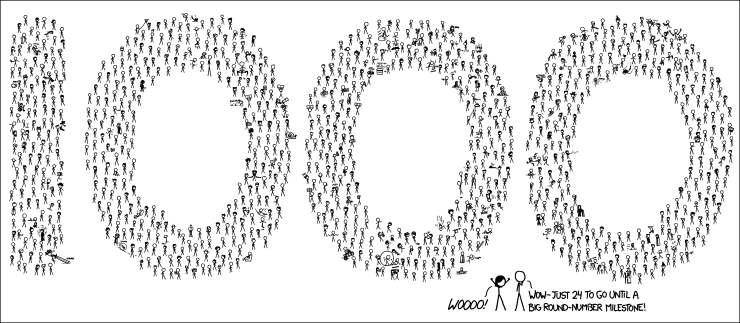
\includegraphics[width=.9\linewidth]{./gfx/xkcd-1000}
%\end{center}
%\captionof{figure}
%	[Dezimale und binäre runde Zahlen]
%	{Dezimale und binäre runde Zahlen. Quelle: \url{https://www.xkcd.com/1000/}}
%\end{hintbox}
